% !TEX TS-program = xelatex
% !TEX encoding = UTF-8

% This is a simple template for a XeLaTeX document using the "article" class,
% with the fontspec package to easily select fonts.

\documentclass[11pt]{report} % use larger type; default would be 10pt
\usepackage{fontspec} % Font selection for XeLaTeX; see fontspec.pdf for documentation
\defaultfontfeatures{Mapping=tex-text} % to support TeX conventions like ``---''
\usepackage{xunicode} % Unicode support for LaTeX character names (accents, European chars, etc)
\usepackage{xltxtra} % Extra customizations for XeLaTeX
% \fontspec{"[DroidSerif.ttf]"}
% \setmainfont{Droid Serif} % set the main body font (\textrm), assumes Charis SIL is installed
%\setsansfont{Deja Vu Sans}
%\setmonofont{Deja Vu Mono}
\usepackage{amsmath}
\usepackage{xfrac}
% \usepackage{xfrac,unicode-math}
% \setmathfont[version=cambria]{Cambria Math}
% \mathversion{cambria}
\usepackage{cleveref}
\usepackage{epstopdf}
\usepackage{amsmath}
\usepackage{hyperref}
\usepackage{xspace}
\usepackage{mathtools}
\usepackage{tikz}
\usepackage{epsfig}
\usepackage{float}
\usepackage{natbib}
\usepackage{subfigure}
\usepackage{setspace}
\usepackage{tabularx,ragged2e,booktabs,caption}
\usepackage{wrapfig}

% other LaTeX packages.....
\usepackage{geometry} % See geometry.pdf to learn the layout options. There are lots.
\geometry{letterpaper} % or letterpaper (US) or a5paper or....
%\usepackage[parfill]{parskip} % Activate to begin paragraphs with an empty line rather than an indent

\usepackage{graphicx} % support the \includegraphics command and options
\newcommand{\IDK}{*** I DON'T KNOW THIS WORD***}

\title{237D Fusion Technology \\
Handout v. 9.1}
\author{Professor Mohamed Abdou}
%\date{} % Activate to display a given date or no date (if empty),
         % otherwise the current date is printed 


\begin{document}
\maketitle
\chapter{Radiation Damage in FW/Blanket Structural Materials and Superconducting Magnet Materials}

\section{Page 2}
\subsection{Structural materials}
\begin{itemize}
\item First wall
\item Blanket
\item Other components
\end{itemize}
Candidates: SS, FS, V-alloy, Nb-alloy, M-alloy

Key Problems:
\begin{enumerate}
\item Radiation damage by intense neutrons
\item Radioactivity
\end{enumerate}

For First Wall:
Additional problem:
Surface effects: Intense bombardments by charged particles (H,$\alpha$, impurities) result in surface erosion (sputtering physical \& chemical, blistering, etc.)

For the next two lectures, we will focus on radiation damage and radioactivity issues.

\section{Page 3}
Additional definitions:

\begin{equation}
	\text{Fluence} \equiv \Phi t_{op}
\end{equation}

\begin{equation}
  \Phi = \text{neutron flux}
\end{equation}

\begin{align}
  t_{op} & = \text{exposure time} \\
         & = \underbrace{\text{time elapsed}}_{t} \times \underbrace{\text{availability}}_{F}
\end{align}

\begin{equation}
	F = \text{plant availability} = \frac{\text{operating time}}{\text{operating time + shutdown time}}
\end{equation}
% Integrated neutron wall load
\begin{align}
  I_w & \equiv \text{Integrated Neutron Wall Load} \\
      & = P_{nw} \times t_{op},  \qquad \qquad [\text{MW y/m}^2] \\
      & = P_{nw} \times t \times F
\end{align}

% \begin{align}
% I_w &= P_{nw} t_{op},  \qquad \qquad [MW y/m^2]     \\
%   	&= P_{nw} t F
% \end{align}

Commonly we measure first wall life in units of MW y/m$^2$
% Aspect Ratio for a tokamak $\equiv A$.

\begin{align}
  A & \equiv \text{Aspect Ratio for a tokamak} \\
    & = \frac{\text{(plasma) major radius}}{\text{(plasma) minor radius}} \\
    & = \frac{R_0}{a}
\end{align}

% \begin{equation}
% 	A = \frac{\text{(plasma) major radius}}{\text{(plasma) minor radius}}
% \end{equation}

\begin{figure}[!htp]
  \centering
  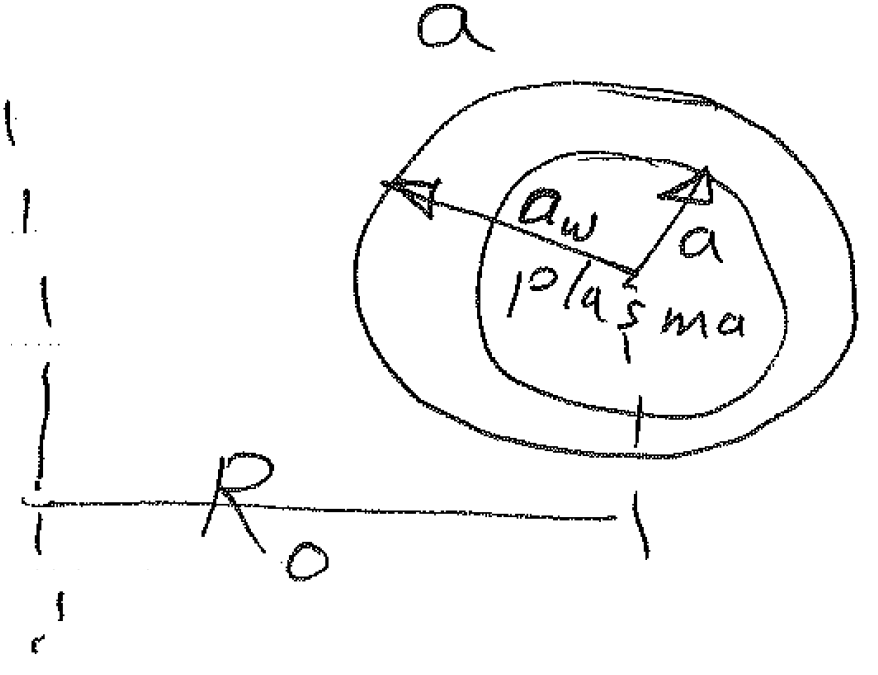
\includegraphics[width=0.45\textwidth]{sketches/sketch1.png}
  \caption[width=\textwidth]{Major and minor radius of toroidal reactor}
  \label{fig:reactorRadius}
\end{figure}

\section{Page 4}

\subsection{Radiation Damage}
Units

Flux \& Fluence poor measure
Total flux ~ a factor of 10 higher than 14 MeV neutron current

neutron spectrum provides improvement but it is awkward.

Useful units: dpa

\IDK

Gas production (He,H)

Important for different \IDK mechanics  but both are \IDK for synergistic effects.
appm for transmutation products

\subsection{Atomic Discplacements}
An energetic particle such as a neutron looses its energy either by electronic excitation or by colliding with the lattice atoms. In a collision with the lattice atom an some energy is transferred into this atom if the quantity of energy transferred is larger than the energy binding the atam in its lattice the stuck atom is displaced by the bombarding particle is called the \textit{primary knock-on atom}, (PKA). Become the PKA possesses substantial kinetic energy, it becomes an energetic particle in it own right

\section{Page 5}
and is capable of creating additional lattice displacements. A displaced atom leaves (i.e. a point defect) its proper place leaving a vacancy behind. The displaced atom will eventually appear in the lattice as an interstitial atom (a point defect). The ensemble of point defects created by a single primary knock-on atom is known as \textit{displacement cascade}.

\subsection{Atomic Displacements Calculating}
\begin{equation}
	\text{dpa} = \text{number of displacements per atom}
\end{equation}
\begin{equation}
	\text{dpa} = \left[ \int \Phi(E) \sigma_d (E) dE \right] t_{\text{radiation time}}
\end{equation}
\begin{equation}
	\sigma_d = \text{displacement cross section}
\end{equation}
\begin{equation}
	\sigma_d(E) = \sum_{\text{all collisions}} \text{probability that a collision occurs} \times \text{the number of atoms displaced by the PKA}
\end{equation}

\section{Page 6}
\begin{equation}
	\sigma_d(E) = \sum_{\text{all \IDK}} \sigma_e (E) \int_{E_d}^{T_{max}} P_i(E,T) \nu(T) dT
\end{equation}
\begin{equation}
	\sigma_i = \text{(nuclear) microscopic cross section for reaction i (elastic, inelastic, (n,2n), (n,$\alpha$), etc.)}
\end{equation}
\begin{equation}
	P_i(E,T) = \text{probability that in reaction i induced by a particle (neutron) of energy E, the PKA has a kinetic energy T}
\end{equation}
\begin{equation}
	E_d = \text{displacement energy or the displacement threshhold}
\end{equation}
\begin{equation}
	\nu(T) = \text{number of displacements produced by a primary knock-on with energy T}
\end{equation}

\subsection{Discussion of \texorpdfstring{$E_d$}{}}
In order for the atom to be displaced it must receive a minimum amount of energy. This is called the displacement energy or the displacement threshold, $E_d$. If the energy transfer $T$ is $<E_d$, the stick atom undergoes large amplitude vibration without leaving the partical well forming its stable lattice portion. The vibration energy is quickly

$E_d$ is in the range of 20 to 60 eV for ()

\section{Page 7}
communicated to the nearest neighbors of the stuck atom and appears as a localized source of heat. On the other hand, if $T>E_d$, the stuck atom is able to pass over the potential barrier and move off into the lattice as a displaced atom.

\begin{wrapfigure}{r}{0.5\textwidth}
  \begin{center}
  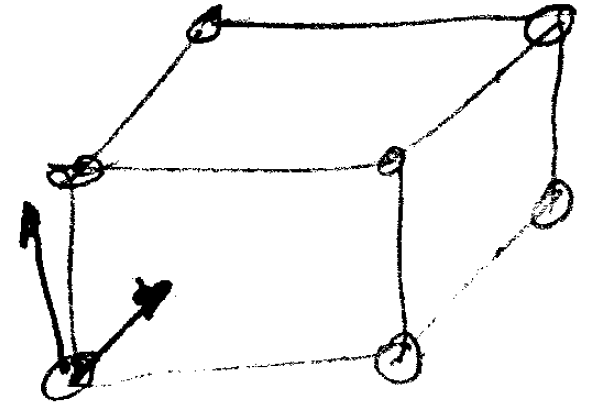
\includegraphics[width=0.45\textwidth]{sketches/sketch2.png}
  \end{center}
  \caption{Diagram of lattice}
\end{wrapfigure}

In a solid, the potential barrier surrounding a lattice atom in its equilibrioum position \textit{is not uniform} in all directions. Therefore, the energy required to displace an atom depends on the \textit{direction} of the recoil. The direction acquired by the recoil is, of course, dictated by the dynamics of the reactions. In the case of isotropy (isotropic collisions, or high number of bombarding particles that collide isotropically) the direction of the recoil is random or equally probable in all directions.

Therefore, the single value of $E_d$ employed in radiation damage theory is \textit{the spherical average of} $E_d(\theta)$ surrounding the equilibrium lattice site, $E_d$, of course, varies from one material to the other but is generally in the range of 20-60 eV.

\section{Page 8}
$\nu(T)$ is the number of displacements produced by a PKA with energy $T$. The value of $\nu(T)$ should be \textit{independent of the type of collision that produced the PKA}. The crux of the damage producing effect of fast neutrons is the production of displaced atoms by the primary knock-ons. Therefore the calculation of $\nu(T)$ is a very important part of the radiation damage theory.

\begin{wrapfigure}{r}{0.5\textwidth}
  \begin{center}
  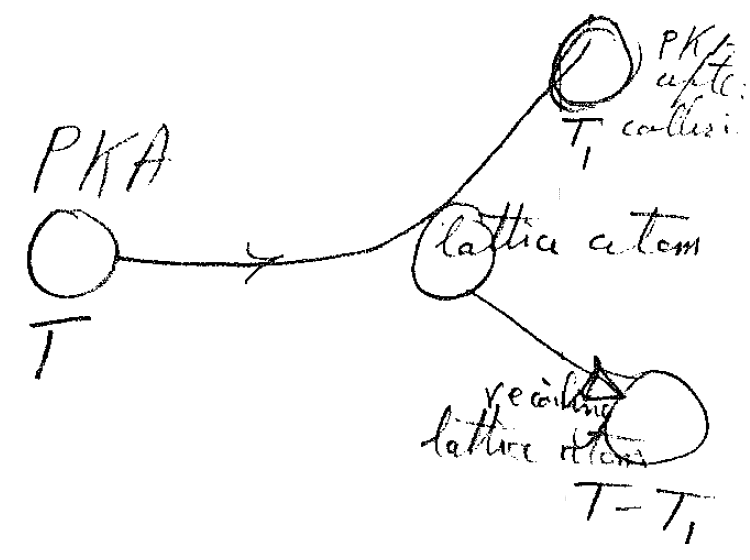
\includegraphics[width=0.35\textwidth]{sketches/sketch3.png}
  \end{center}
  \caption{PKA collision with lattice}
\end{wrapfigure}

There are several models that have been developed to calculate $\nu(T)$. These models \IDK in the assumptions invoked. However, almost all of them heat the interaction between \IDK a moving atom and the lattice atoms as a sequence of two-body elastic collisions.

There are two important observations you should be aware of regarding this assumption of two-body collisions and elasticity.

\section{Page 9}
\subsection{Handwritten}
The primary collision assumption is quite satisfactory at high interaction energies because the approach distance giving substantial energy transfer are very much smaller than the distances between lattice atoms, \IDK the collisions can be considered to occur between isolated pairs of atoms. However, at low energies appoaching the threshold $E_d$, the cross section for atom-atom interaction is large, and the incoming atom can interact with more than one atom at the same time.

\subsection{Typed}
The collision between a recoil and a lattice atom is often assumed to be elastic, which means that kinetic energy is conserved in the event. Inelasticity can arise from excitation or ionization of the orbital electrons of the atoms involved in the collision. Indeed, interaction of moving atoms or ions with the electrons of the solid constitute the major energy-loss process at high energies. Transfer of energy from the moving atom to electrons does not lead to displacement, only to heat; the low electron mass means that they carry little momentum even though they may be quite energetic. Consequently, it is important to be able to estimage the degree to which the energy of a recoil atom is partitioned between electronic excitation and elastic atom-atom collisions. Only the energy transferred in the latter process is available for causing displacements. Energy is transferred to the electrons in small increments so closely spaced that the process can be regarded as a continuous loss of energy by the moving atom. The atom continues to travel in a straight line but slows down as if it were passing through a viscous medium. The atom-atom interactions, on the other hand, occur at widely spaced intervals; transfer a significant portion of the initial kinetic energy of the moving atom in an essentially instantaneous collision, and produce substantial deflections of the original energetic atom. Consequently, the total energy loss of a moving atom can be accurately separated into two parts: (1) discrete elastic atom-atom encounters which both reduce the energy of the incident atom and produce lattice displacements and (2) a continuous process of electronic excitation which contributes to energy loss but not to displacements.

Not all the energy transferred to a stationary lattice atom by a recoil atom by process 1 is used to displace the former. A substantial portion of the initial energy of the PKA is degraded to heat by atom-atom collisions that do not deliver the requisite displacement energy to the struck atom. In this event the struck atom simply rattles about in its lattice site, ultimately degrading the energy it recieved in the collision to heat.

\section{Page 10}

\section{Typed (on a typewriter)}

The helium or hydrogen production rate in material j due to nuclear transmutation can be calculated from

\begin{equation}
	R_{\alpha}(\vec{\mathbf{r}}) = \int N_j(\vec{\mathbf{r}}) \sigma_{(n,\alpha)j}(E)_{\phi}(\vec{\mathbf{r}},E) dE
\end{equation}
and
\begin{equation}
	R_{H}(\vec{\mathbf{r}}) = \int N_j(\vec{\mathbf{r}}) \sigma_{(n,p)j}(E)_{\phi}(\vec{\mathbf{r}},E) dE
\end{equation}
The helium and hydrogen production rate distributions per 14 MeV neutron leaving the plasma that were calculated for representative blankets are shown in Figures 9.4.2 and 9.4.3.

The helium and hydrogen concentration are commonly expressed in terms of the number of He or H atoms per million lattice atoms, or in atomic parts per million (appm).

Table 9.4.1 summarizes the displacements and He and H concentrations that would result from a neutron fluence of 1 MW y/m$^2$ $(4.48\times 10^{17}$ 14 MeV neutrons per m$^2$) incident upon various materials.
\begin{table}
\centering
\begin{tabular}{|lccc|}
\hline
Material & dpa & appm He & appm H \\
\hline
316SS & 10 & 200  & 540   \\
Nb    & 7  & 24   & 79    \\
Mo    & 8  & 47   & 95    \\
V     & 12 & 57   & 100   \\
C     & 10 & 2700 & small \\
Be    &    & 2800 & 130   \\
\hline
\end{tabular}
\caption{Primary Response Characteristics (Neutron Fluence of 1 MW y/m$^2$)}
\end{table}

\newpage
\section{Pages 11-14}

\begin{figure}[h!]
  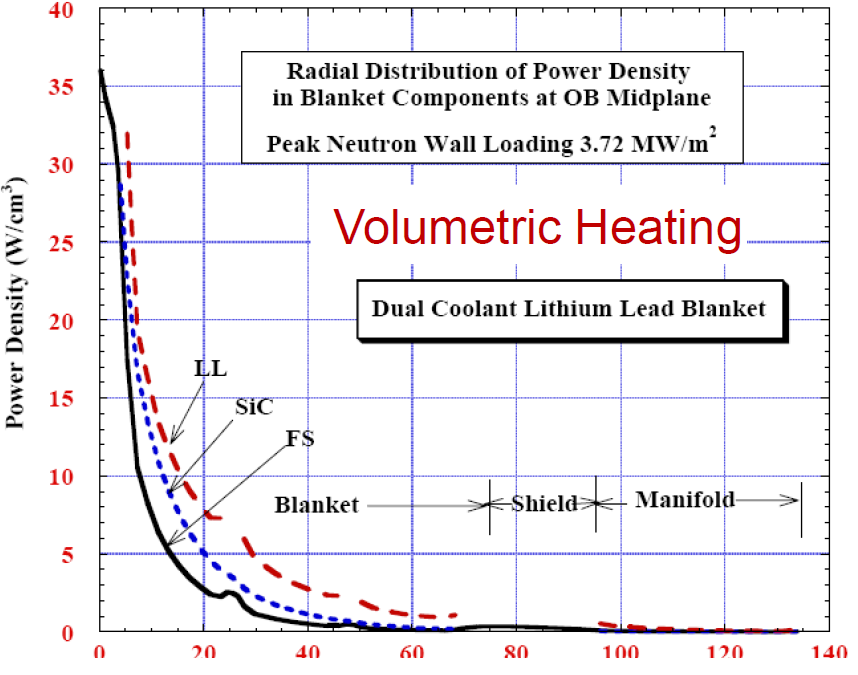
\includegraphics[width=0.45\textwidth]{figs/PowerDensity.png}
  \label{fig:PowerDensity}
  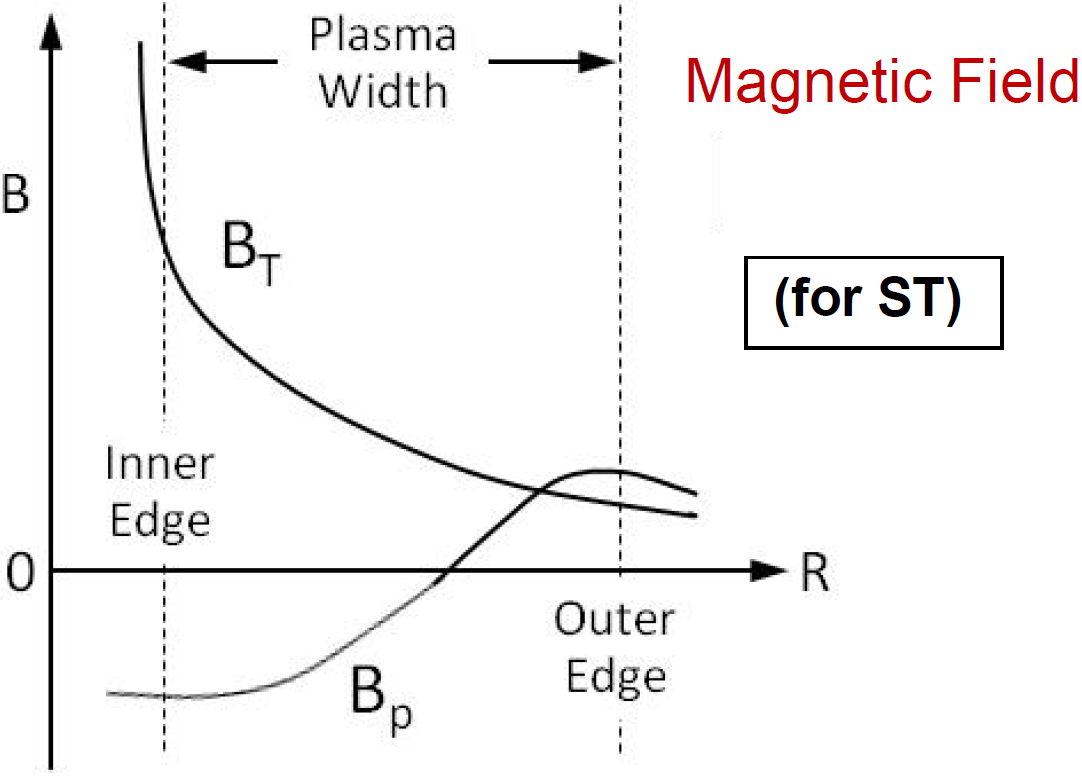
\includegraphics[width=0.45\textwidth]{figs/Bfield.png}
  \label{fig:Bfield}
  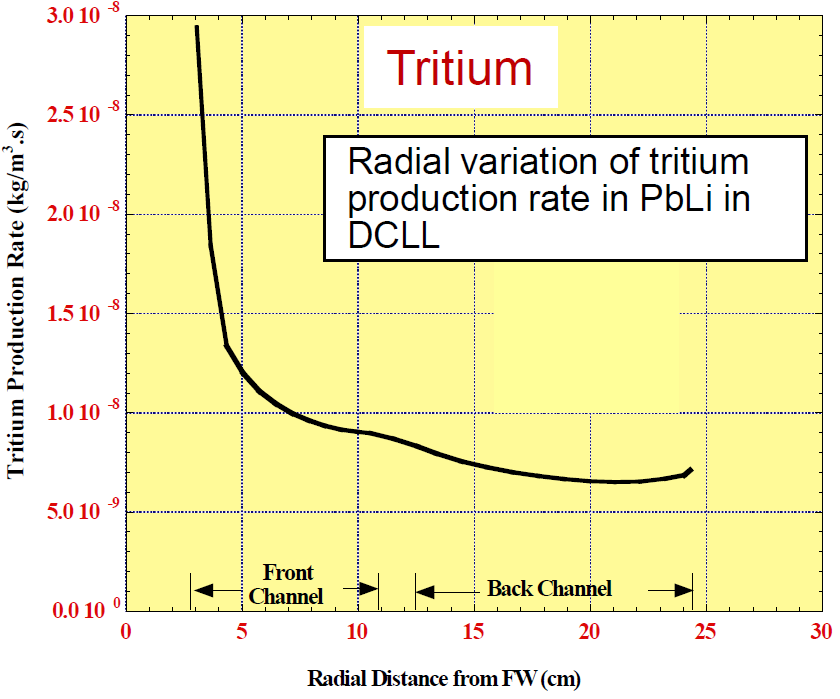
\includegraphics[width=0.45\textwidth]{figs/tritiumProduction.png}
  \label{fig:tritiumProduction}
  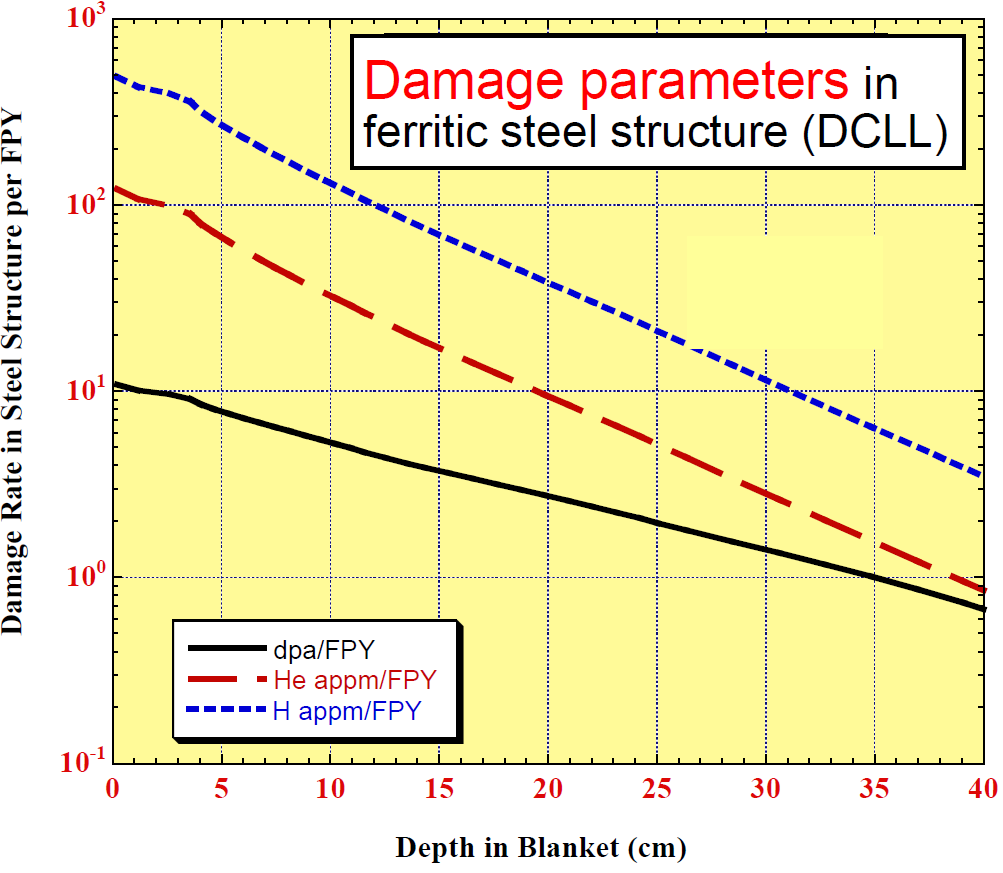
\includegraphics[width=0.45\textwidth]{figs/damageParameters.png}
  \label{fig:damageParameters}
  \caption{PKA collision with lattice}
\end{figure}

\begin{figure}[h!]
  \centering
  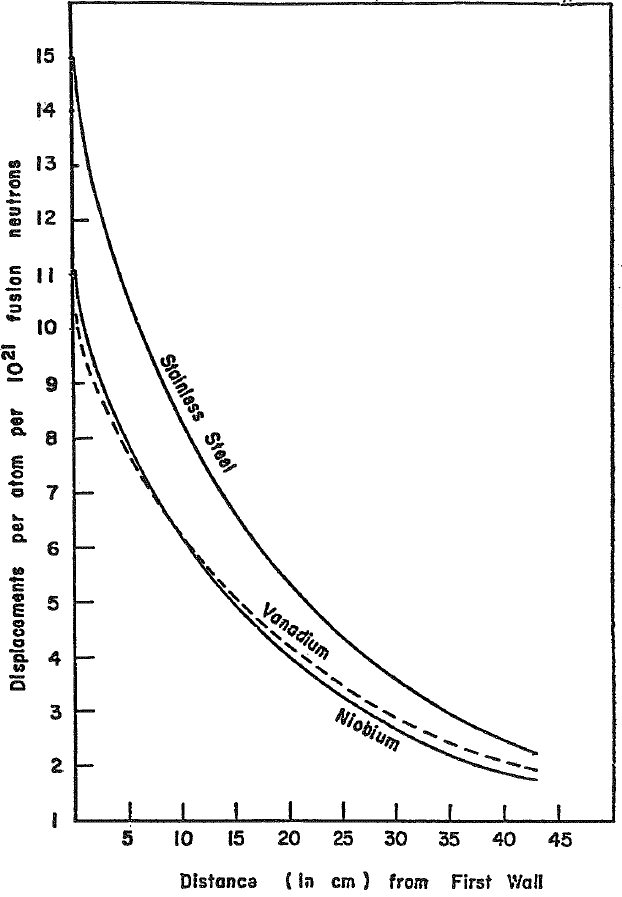
\includegraphics[width=0.45\textwidth]{figs/dpa.png}
  \caption{Comparison of Atomic Discplacement for Vanadium, Niobium and Stainless Steel}
  \label{fig:dpa}
\end{figure}
\begin{figure}[h!]
  \centering
  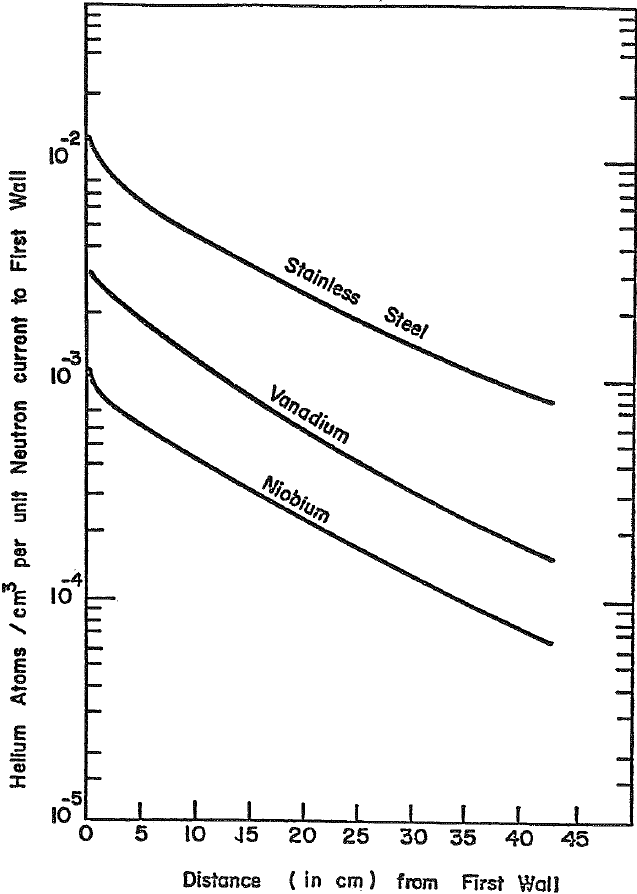
\includegraphics[width=0.45\textwidth]{figs/HeProduction.png}
  \caption{Comparison of Helium Production in Vanadium, Niobium and Stainless Steel}
  \label{fig:HeProduction}
\end{figure}
\begin{figure}[H]
  \centering
  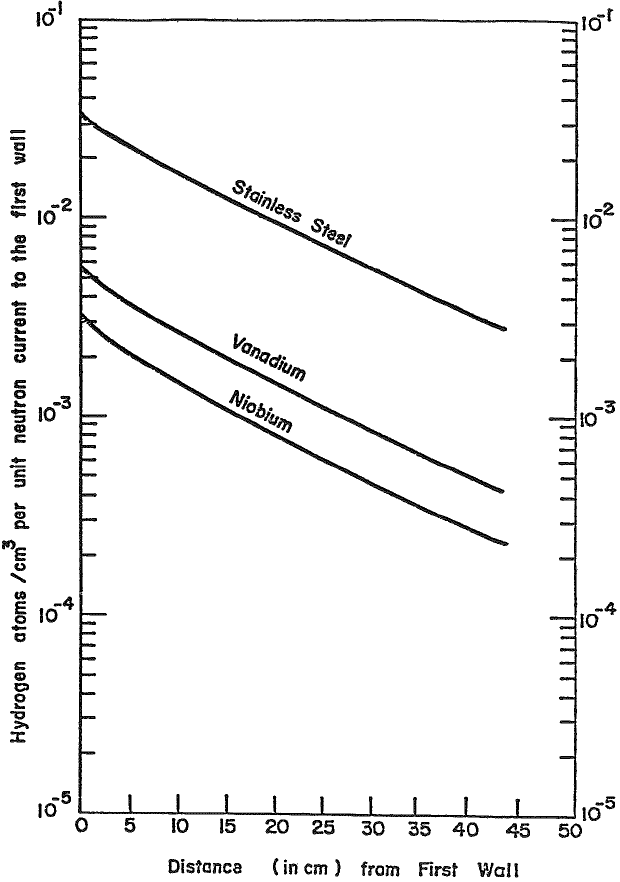
\includegraphics[width=0.45\textwidth]{figs/HProduction.png}
  \caption{Comparison of Hydrogen Production in Vanadium, Niobium and Stainless Steel}
  \label{fig:HProduction}
\end{figure}

\section{Page 15}
\subsection{Material Properties Changes (radiation effects)}
The primary responses (displacements and transmutations) cause changes in the ephysical and mechanical properties of materials that are subjected to neutron bombardment. These secondary responses are indicated in Table \ref{fig:table2}.

% \begin{table}[h!]
% \centering
% \begin{tabular}{|c|c|}
%   \hline
%   Primary Response & Secondary Response \\
%   \hline
%   Displacements & Swelling \\
%   Transmutations & Dimensional instabilities \\
%   \hline
% \end{tabular}
% \caption{Physical and Mechanical Property Changes} \label{tab:phys}
% \end{table}

\begin{figure}[h!]
  \centering
  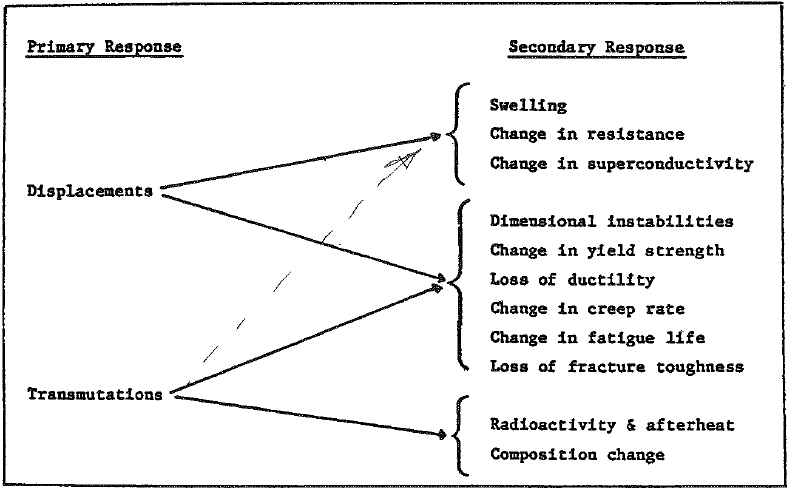
\includegraphics[width=0.45\textwidth]{tables/table2.png}
  \caption{Physical and Mechanical Property Changes}
  \label{fig:table2}
\end{figure}

The properties of structural materials are affected by neutron radiation in many different ways. Displacements produce interstitial atoms and lattice vacancies in pairs. The interstitials are highly mobile and insoluble, so that they tend to form loops, leaving an excess of vacancies in the lattice. These vacancies precipitate into 

\section{Page 16}
three-dimensional voids if the temperature is sufficiently high and if there are nucleation sites. This microstructural change has no macroscopic effect until after a certain threshold dpa level has been reached, after which the material begins to swell. After the incubation dose has been exceeded, the volumetric swelling in structural materials increases linearly with dpa. The projected swelling rate for a modified stainless steel is shown in Figure \ref{fig:swelling}. The swelling characteristics are material- and temperature-dependent.

Hardening of the lattice matrix in the grains of metals due to displacements causes deformation to occur along grain boundaries under stress. Helium collects on the grain boundaries, aggravating the problem by interferring with grain boundary sliding, which would otherwise relieve the stress. This process produces microcracks which eventually lead to fracture. One measure of ductility is the percentage of tensile elongation that is permissible without fracture. The effect of neutron radiation damage upon the tensile elongation of 316 stainless steel is dipicted in Figure \ref{fig:elongation}. 

Defects caused by displacements can act as barriers to dislocation motion, causing metals to become stronger. The yield strength of austenitic stainless steels will generally increase under neutron irradiation by as much as a factor of ~3.

Materials under thermal stress tend to slowly deform to relieve that stress, a process known as thermal creep. Neutron radiation has been observed to enhance the normal thermal creep rate. The additional "irradiation" creep is proportional to dpa.

When a structural material is repetitively cycled under a loading that produces a strain $\varepsilon$ it will eventually fail. The number of cycles to failure is directly related to the magnitude of the strain. When a material is irradiated with neutrons, this "fatigue" lifetime is decreased, as illustrated in Figure \ref{fig:fatigueLife}.

If a small flaw exists in a structural component, that flaw will grow under a cyclic loading until fracture takes place. The fracture mechanism is plastic instability on a local scale. The resistance to flaw growth can be characterized by a parameter known as fracture toughness. Neutron radiation reduces the fracture toughness of structural materials.

\section{Pages 17}

\begin{figure}[H]
  \centering
  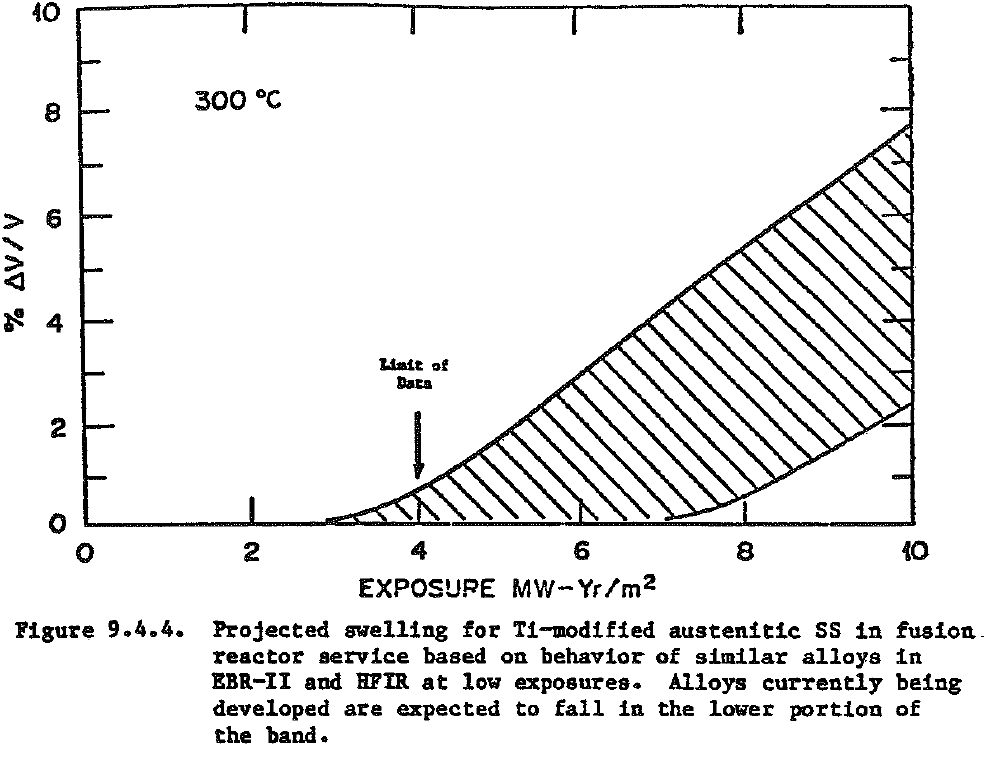
\includegraphics[width=0.45\textwidth]{figs/swelling.png}
  \caption{Projected swelling for Ti-modified austenitic SS in fusion reactor service based on behavior of similar alloys in EBR-II and HFIR at low exposures. Alloys currently being developed are expected to fall in the lower portion of the band.}
  \label{fig:swelling}
\end{figure}

\begin{figure}[H]
  \centering
  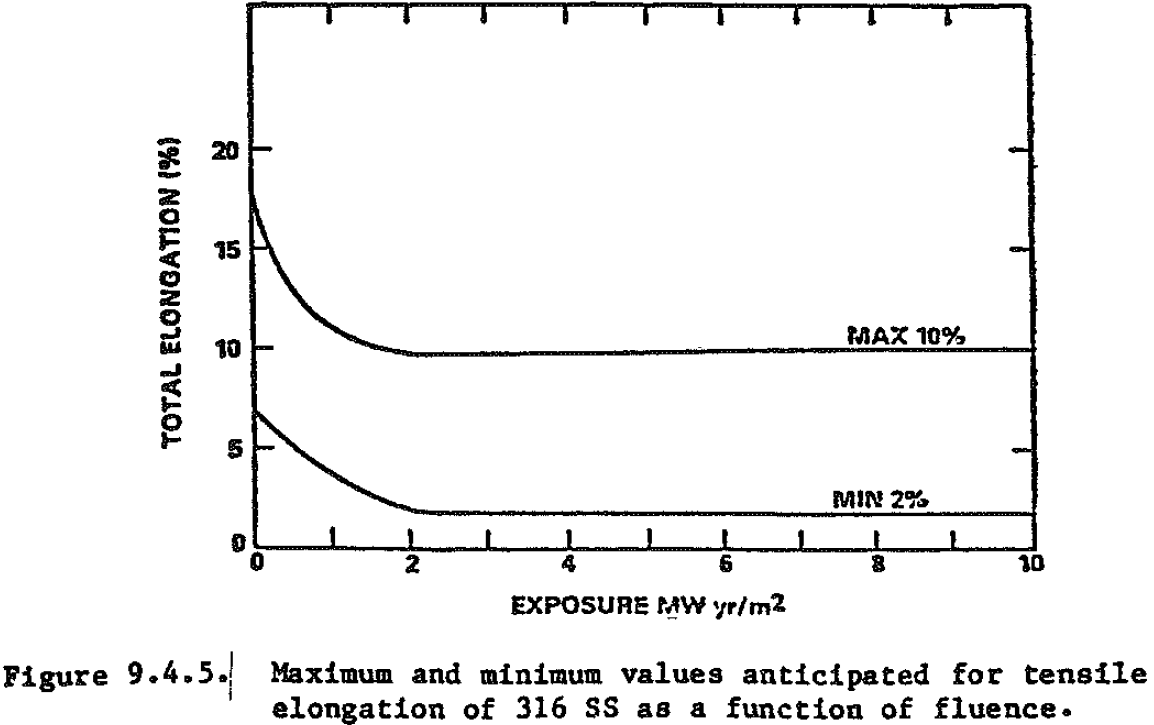
\includegraphics[width=0.45\textwidth]{figs/elongation.png}
  \caption{Maximum and minimum values anticipated for tensile elongation of 316 SS as a function of fluence.}
  \label{fig:elongation}
\end{figure}

\section{Pages 18}

\begin{figure}[H]
  \centering
  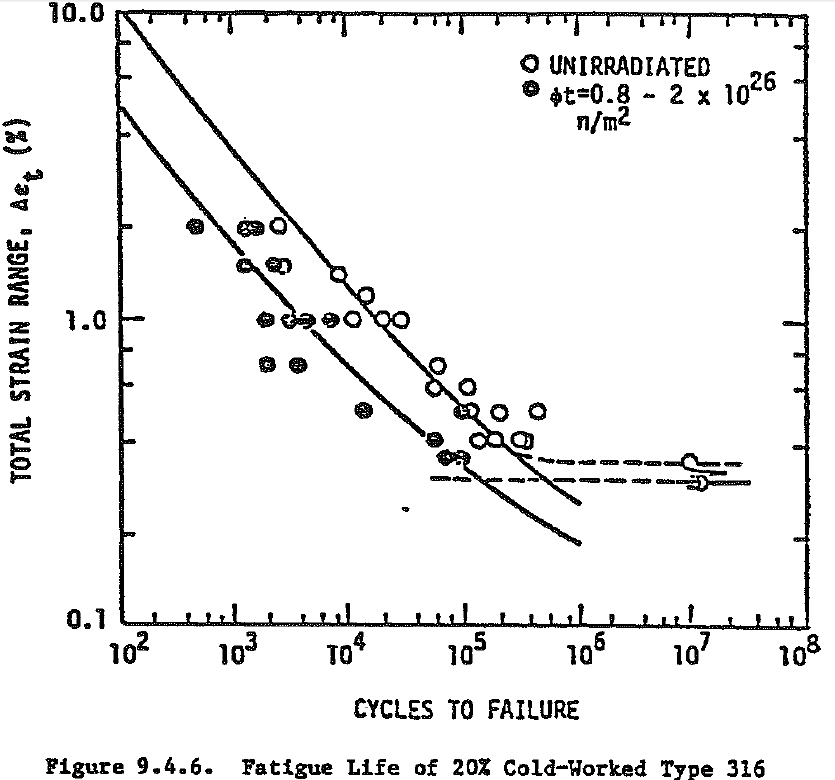
\includegraphics[width=0.45\textwidth]{figs/fatigueLife.png}
  \caption{Fatigue Life of 20\% Cold-Worked Type 316}
  \label{fig:fatigueLife}
\end{figure}

\begin{figure}[H]
  \centering
  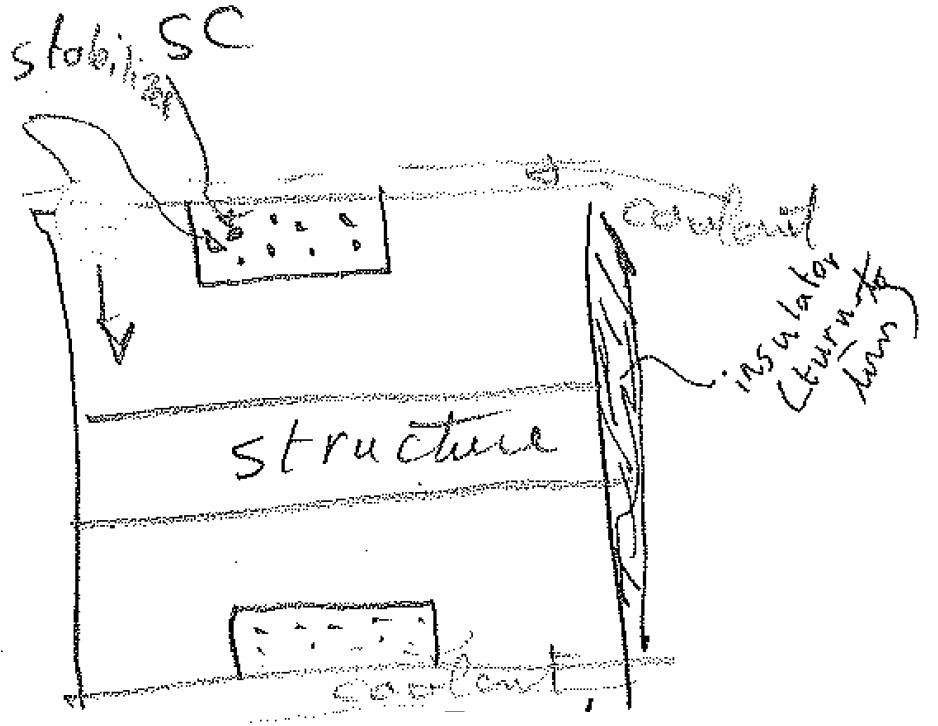
\includegraphics[width=0.45\textwidth]{sketches/sketch4.png}
  \caption{Sketch of .}
\end{figure}

\begin{figure}[H]
  \centering
  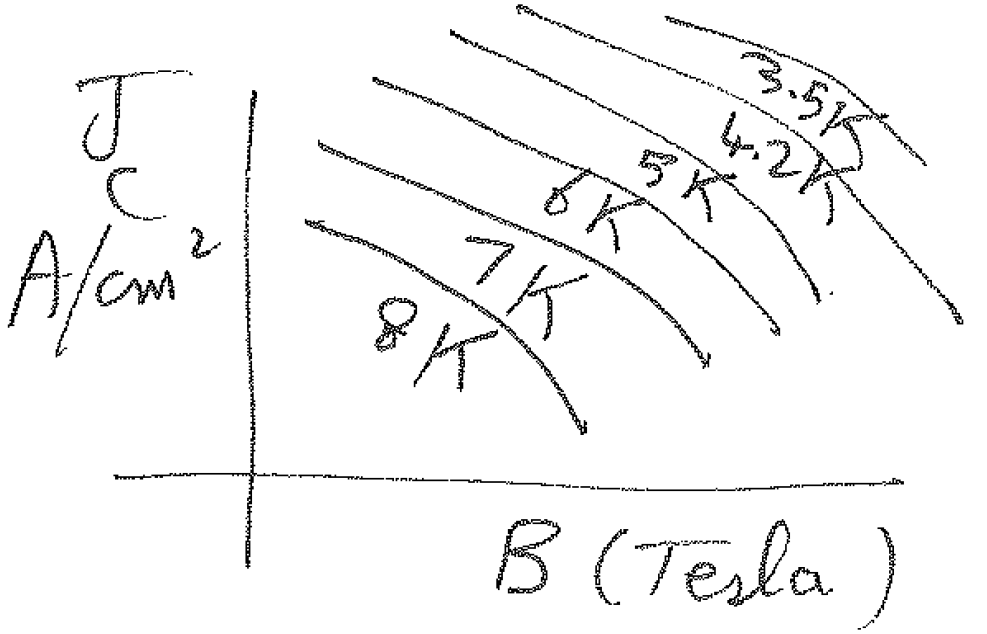
\includegraphics[width=0.45\textwidth]{sketches/sketch5.png}
  \caption{Sketch of vs magnetic field for various temperatures.}
\end{figure}

Superconducting magneti components are adversely affected by radiation also. The effect of neutron radiation on the superconductor itself is to diminish the superconducting region of current density-temperature-magnetic field phase space. The critical current density of Nb$_3$Sn has been observed to change above ~$1.5\times 10^{-3}$ dpa ($3\times 10^{22}$ n/m$^2$). The effect is much less pronounced for NbTi, with a decrease of less than a factor of 2 being observed at fluences up to $10^{24}$ n/m$^2$. These data are shown in Figure \ref{fig:irradiationEffect}.

\section{Page 19}

\begin{figure}[H]
  \centering
  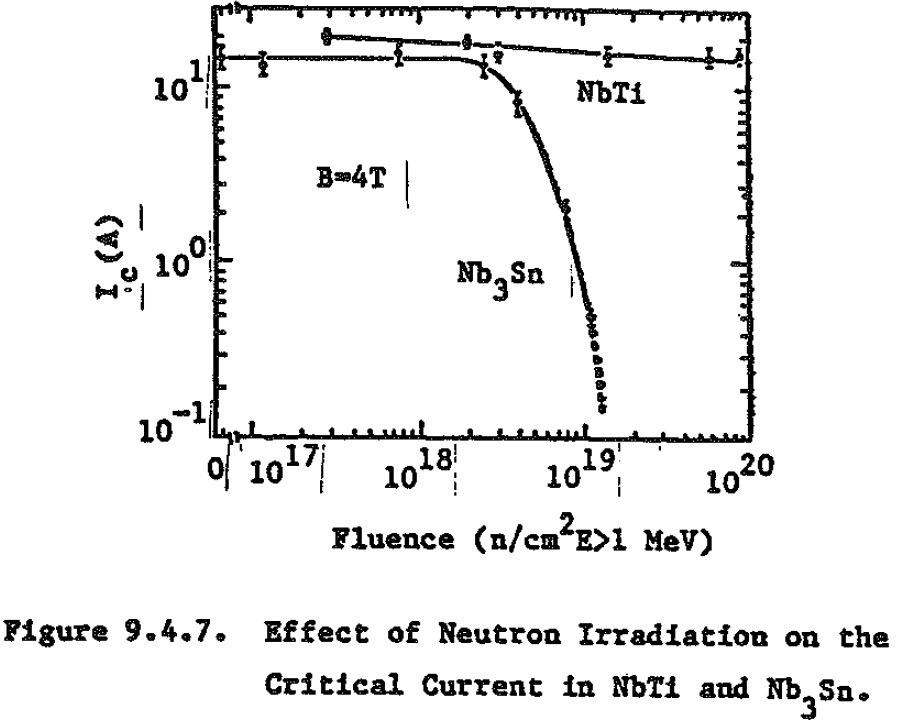
\includegraphics[width=0.45\textwidth]{figs/irradiationEffect.png}
  \caption{Effect of Neutron Irradiation on the Critical Current in NbTi and Nb$_3$Sn.}
  \label{fig:irradiationEffect}
\end{figure}

The resistance of normal conductors, which are used for cryogenic stability, at 4.2 K increases dramatically with dpa, as illustrated in Figure \ref{fig:resistivity}.

\underline{Additional handwritten notes}
For NbTi
\begin{equation}
  J_c = J_{c0} e^{-\alpha \phi t}
\end{equation}
$\alpha = 3.5 \times 10^{-24}$ m$^2$ at $\phi t \sim 3 \times 10^{22}$ n/m$^2$.
$\frac{\Delta J_c}{J_c} \sim 10\%$

\begin{equation}
  J \bullet A_{\text{cross section}} = I
\end{equation}
Need for a stablizer
\begin{equation}
  I^2 R \le q'' P_{\text{cooled perimeter}} l
\end{equation}
\begin{equation}
  I^2 \rho \le q'' P l
\end{equation}
\begin{equation}
  I^2 \rho \le q'' Pa
\end{equation}

\begin{equation}
  \rho = \rho_0 + \rho_{\text{magnetic field}} + \rho_{\text{radiation}}
\end{equation}

$\rho_{\text{magnetic field}} = 4.55 \times 10^{-9}$ tesla $\Omega$cm

$2-5 \times 10^9$ rad
1 rad $\sim 10^9$ n/cm$^2$ $\sim 10^13$ n/m$^2$

\begin{figure}[H]
  \centering
  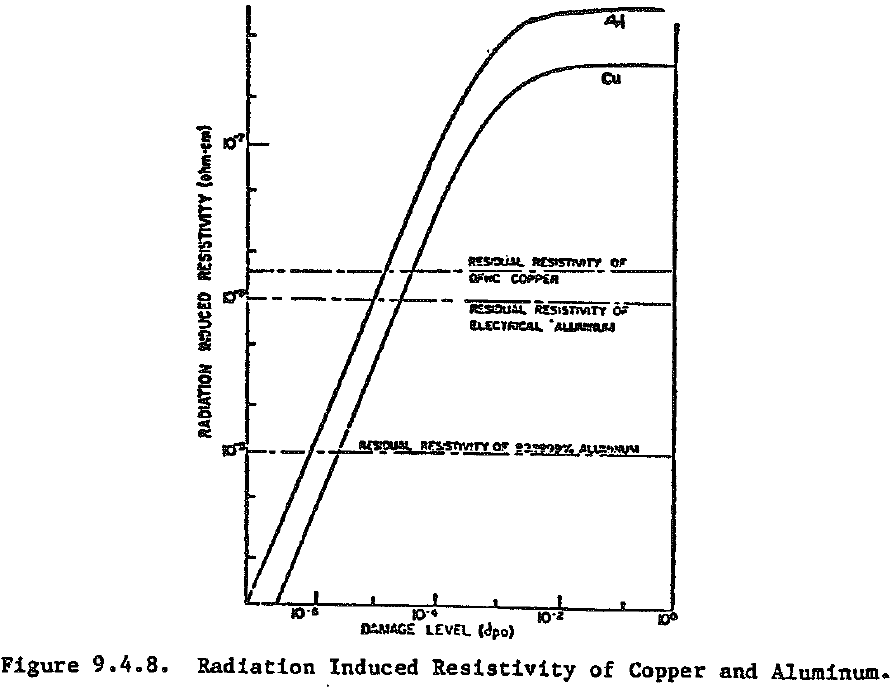
\includegraphics[width=0.45\textwidth]{figs/resistivity.png}
  \caption{Radiation Induced Resistivity of Copper and Aluminum.}
  \label{fig:resistivity}
\end{figure}

The organic insulators that are used in superconducting magnets have been observed to physically deteriorate from neutron damage in the range 2-5$\times 10^{22}$ n/m$^2$. Inorganic insulators, on the other hand, retain their physical properties up to damage in excess of $10^{25}$ n/m$^2$. However, the inorganic insulators are brittle. There are indications that neutron radiation-induced microstructural change in granular solid breeding materials (see Section 10.1) may significantly reduce the tritium release properties. Tritium trapping at radiation-induced defects could be significant. Radiation-induced sintering could lead to reduction in porosity, which would reduce the tritium migration. The size of the basic grains could grow under radiation, leading to reduced tritium diffusion out of the grains in which it is produced.

\subsection{Radioactivity (crossed off)}
Many of the new isotopes produced by nuclear transmutations following neutron capture (e.g. (n,$\gamma$), (n,$\alpha$), (n,p), (n,2n)) are unstable and will, over a period of time, decay by the emission of a charged particle. The resulting isotope may itself be unstable and undergo further decay, thus leading to a so-called decay-chain. The nuclide densities of the isotopes in a given decay chain are described by the set of equations

\begin{equation}
  \frac{d N_i(\vec{\mathbf{r}},t)}{dt} = 
  - (\lambda_i + \overline{\sigma}_i \overline{\phi}(\vec{\mathbf{r}})) N_i(\vec{\mathbf{r}},t) +
  \sum_{j \ne i}^{J} (\lambda_j + \overline{\sigma}_{j-i} \overline{\phi}(\vec{\mathbf{r}})) N_j(\vec{\mathbf{r}},t),
  \qquad i=1,...,J
\end{equation}

Here, $\lambda_i$ is the radioactive decay constant for isotope $i$ and $\alpha_{j \rightarrow i}$ is the probability that the decay of isotope $j$ leads to isotope $i$ (e.g.) if the

\end{document}